\documentclass[12pt,a4paper,oneside]{report}

% Page layout
\usepackage[a4paper,top=1.7cm,bottom=7.4cm,left=2.5cm,right=6.0cm,footskip=6.3cm]{geometry}
\usepackage{setspace}
\usepackage{titlesec}
\usepackage{titling}
\usepackage{times}
\usepackage{fontspec}
\setmainfont{Arial}
\usepackage{fancyhdr}
\pagestyle{fancy}
\fancyhf{}
\fancyfoot[C]{\thepage}
\renewcommand{\headrulewidth}{0pt}
\renewcommand{\footrulewidth}{0pt}

% Include PDF
\usepackage{pdfpages}
% Bibliography
\usepackage{natbib}
\bibliographystyle{plain}  % or another style that suits your needs
\usepackage{url}
\usepackage{hyperref}
% math
\usepackage{amsmath}

% for Plant Count section
\usepackage{tabularx}         % For tabularx environment
\usepackage{float}            % For H float option
\usepackage{subfig}           % For subfloat command
\usepackage{changepage}       % For adjustwidth environment
\usepackage{booktabs}         % For toprule, midrule, bottomrule commands
\usepackage{cleveref}         % For \cref command


% Paragraph formatting
\setlength{\parskip}{6pt}
\setlength{\parindent}{0pt}
\setstretch{1.5}

% Define extralength parameter
\newlength{\extralength}
\setlength{\extralength}{0cm}

\begin{document}

% Include the first page from the PDF file

\includepdf[pages=1]{Intestazione/t3._Thesis_first_page.pdf}

% Table of Contents
\tableofcontents
\newpage

% Main content
\chapter{Introduction}

\section{Phytosanitary Products}

Phytosanitary products, commonly used as a synonym for "Plant Protection Products" (PPPs),
are a specific category of pesticides designed primarily to maintain crop health 
and prevent destruction by diseases and infestations. While the term "pesticides" 
is broader and also includes biocidal products used to control harmful organisms 
and disease carriers not related to plant protection, phytosanitary products are 
specifically used to control harmful organisms affecting cultivated plants (such 
as insects, mites, fungi, bacteria, rodents, etc.), eliminate weeds, and regulate 
plant physiological processes. Fertilizers, which serve for plant nutrition and 
soil fertility improvement, are excluded from phytosanitary products.

Phytosanitary products contain at least one active substance, which can be either 
chemical compounds or microorganisms, including viruses, that enable the product 
to perform its intended function. These active substances undergo rigorous risk 
assessment processes, with EFSA (European Food Safety Authority) playing a central 
role in conducting peer reviews at the EU level to determine if these products, 
when used correctly, might produce harmful effects on human or animal health, either 
directly or indirectly through drinking water, food, or feed.

The main categories of phytosanitary products can be distinguished based on the 
type of organism they target or the function they perform, including:


\begin{itemize}
    \item Fungicides
    \item Insecticides
    \item Acaricides
    \item Rodenticides
    \item Slimicides
    \item Nematicides
    \item Herbicides
    \item Plant growth regulators
\end{itemize}

The parameters identified through the risk assessment are compared with the values 
established by directive 97/57/EC \cite{EURLex1997265}, which indicates the acceptability limits for 
decision-making on the inclusion of active substances in the EU list (Annex I of 
directive 91/414/EEC \cite{directive_91_414_EEC}).

The Introduction of a product in the EU market is not only subject to audits on
active substances and their safety for humans and environment but also to the evaluation 
of the product's efficacy and safety for the crop.
World Trade Organization Sanitary and Phytosanitary Measures Agreement \cite{WTO_SPS_Agreement}
recognizes the International Plant Protection Convention (IPPC) as the only international
institution in charge of emitting standards for plant health \cite{IPPC}. IPPC is organized in
regions. European Union (EU) countries refer to the European and Mediterranean Plant
Protection Organization (EPPO). EPPO Standards are divided into Standards on
Phytosanitary Measures and Standards on PPPs. PPPs standards describe the efficacy
evaluation of PPPs (PP 1) and good plant protection practices. EU Good Experimental
Practices (GEP) units provide
Biological Assessment Dossier (BAD) efficacy trials. GEP units are expected to follow
EPPO PP 1 to assess PPPs selectivity detecting phytotoxicity effects, and efficacy in the
complaint of Regulation (EC) No 1107/2009 of the European Parliament and Council \cite{EC_Regulation_1107_2009}.

\section{EPPO Standards}

Generics on efficacy assessments are reported in PP 1/181(5) \cite{EPPO_PP1_181}, which describes
herbicide, fungicide, bactericide, and insecticide efficacy on the target evaluation.
PP 1/135(4) \cite{EPPO_PP1_135} describes the selectivity assessment procedures, 
in other words: the standard phytotoxicity assessments of PPPs.
The PP 1/152 \cite{EPPO_PP1_152} standard describes the general principles for the
efficacy and selectivity evaluation of PPPs, in describing the standard experimental design.
Aside from the objectives of the study and the description of thesis (treatments), 
the PP 1/152 outlined that a comprehensive experimental design should include a description of:
\begin{itemize}
    \item \textbf{Type of Design}
    \item \textbf{Sampling Method and Measures Units}
    \item \textbf{Statistical Analysis Plan}
\end{itemize}

\subsection{Experimental Design}

EPPO "envisage trials in which the experimental
treatments are the ‘test product(s), reference product(s) and
untreated control, arranged in a suitable statistical design’" \cite{EPPO_PP1_152}.
The experimental design should be randomized, with replications and blocks, and
should include a sufficient number of plots to ensure the statistical power of the
analysis. The number of replications and blocks should be determined based on the
expected variability of the data and the desired level of statistical significance
in respect control and reference thesis. The
randomization of thesis within blocks should be carried out using a suitable
randomization procedure to ensure that the treatments are assigned to plots in a
completely random manner. The key randomization used in phytosanitary product 
evaluations include:

\begin{itemize}
    \item \textbf{Completely Randomized Design (CRD)}: Treatments randomly assigned to 
          experimental units; statistically powerful but only suitable for homogeneous trial 
          areas where environmental variation is minimal.
          
    \item \textbf{Randomized Complete Block Design (RCBD)}: Groups plots into homogeneous 
          blocks with each treatment appearing once per block; controls for environmental 
          heterogeneity across the experimental area.
          
    \item \textbf{Split-Plot Design}: Used when one factor (e.g., cultivation equipment) 
          cannot be fully randomized; creates hierarchy with whole plots and subplots; 
          particularly useful when plot size or equipment constraints exist.
          
    \item \textbf{Systematic designs}: Non-randomized arrangements rarely suitable for 
          efficacy evaluations; may only be appropriate in special cases like varietal 
          trials on herbicide selectivity.
\end{itemize}

When designing phytosanitary product trials, the arrangement of untreated controls 
is critical for proper efficacy assessment. According to EPPO standards, the main 
purpose of untreated controls is to demonstrate adequate pest infestation, without 
which efficacy cannot be meaningfully evaluated. Four distinct arrangements for 
untreated controls exist:

\begin{itemize}
    \item \textbf{Included controls}: The most common approach, where control plots 
    have the same shape and size as treatment plots and are fully randomized within 
    the experimental design. This arrangement is essential when controls 
    will be used in statistical comparisons.
    
    \item \textbf{Imbricated controls}: Control plots are arranged systematically 
    within the trial (between blocks or between treated plots), potentially with 
    different dimensions than treatment plots. These observations are typically 
    not included in statistical analyses but ensure more homogeneous distribution 
    of untreated area effects.
    
    \item \textbf{Excluded controls}: Control plots are established outside the 
    main trial area but in similar environmental conditions. While replication is 
    not essential, it may be beneficial in heterogeneous environments. These observations 
    are generally excluded from statistical analyses.
    
    \item \textbf{Adjacent controls}: Each plot is divided into two subplots, with 
    one randomly selected to remain untreated. This approach is particularly valuable 
    in highly heterogeneous environments but requires specialized split-plot statistical 
    analysis.
\end{itemize}

The selection of control arrangement depends on several factors: whether the control 
will be included in statistical tests (requiring included controls), the degree 
of environmental heterogeneity (adjacent controls are preferred for high heterogeneity), 
and the potential for control plots to interfere with adjacent treatment plots (suggesting 
excluded controls when interference is likely).
The trials type design is critical for the success of the study, as it ensures
that the results are reliable, reproducible, and statistically valid.

\subsection{Sampling Method and Measures Units}

After defining the experimental units through the randomization design choise,
the next step is to define the sampling method and the measures units.
Target and crop-specific standards point out "mode of
assessment recording and measurements" fixing evaluation metrics in two ways:
countable (discrete values) and measurable (continuous values) effects which must be
expressed in absolute values, in other cases, frequency (incidence) and degree
(severity) should be estimated and reported as affected percentage of the individual (ex.
plant or plot) or as proportion within thesis and control expressed in percentage. As
specified by PP 1/152 \cite{EPPO_PP1_152}, classification by ranking (ordinal) and scoring (ordinal or
nominal) is also contemplated. In the case of estimation, rather than count or measure,
PP 1/152 reports "The observer should be trained to make the estimations and his
observations should be calibrated against a standard". Calibration compliance with
standards is ensured by GEP audits. Scoring and ranking scales examples are
published on specific standards or the same PP 1/152. The lack of specific scales lets
trial protocol authors define one inspired in range and intervals by the mentioned
examples or other well-established ones.
GEP units PP 1 assessments are produced by trained and experienced
agronomists or biologists by visual inspection or laboratory analysis. The technician
follows the trial protocol and related EPPO standards during assessment execution. The
technician is critical for accuracy, precision, and repeatability. Sensitivity is determined
by the trial protocol. It depends on expected differences and if a measure, a proportion,
or a scale is used. For instance, in PP 1/93(3) \cite{EPPO_PP1_93} "Efficacy evaluation of herbicides -
Weeds in cereals - Observation on the crop", phytotoxicity color modification could be
measured, or estimated as proportion in respect to the untreated, or scored in EPPO
scale as PP 1/135(4) reports, or a scientifically accepted score as the European Weed
Research Society phytotoxicity damage score \cite{EWRS_score} and other ones.
In general, data types must undergo the classification presented in Table 1.1

\begin{table}[ht]
\caption{Different modes of observation and types of variables}
\label{tab:data_types}
\centering
\begin{tabular}{|l|c|c|c|c|}
\hline
\textbf{Type of Variable} & \textbf{Measurement} & \textbf{Visual Estimation} & \textbf{Ranking} & \textbf{Scoring} \\
\hline
Binary & & & & X \\
\hline
Nominal & & & & X \\
\hline
Ordinal & & & X & X \\
\hline
Discrete & X & X & & \\
\hline
Continuous limited & X & X & & \\
\hline
Continuous not limited & X & X & & \\
\hline
\end{tabular}
\end{table}

\subsection{Statistical Analysis}

The statistical analysis of trials is equally critical, providing objective 
assessment of treatment effects. While PP 1/152 \cite{EPPO_PP1_152} doesn't prescribe 
specific analyses for all situations, it emphasizes that analysis methods should 
align with the experimental design and data types collected. For quantitative 
variables (continuous or discrete), parametric methods based on Generalized 
Linear Models (GLM) are recommended, including ANOVA and regression approaches. 
For qualitative variables (bynary, ordinal or nominal), non-parametric methods are more 
appropriate. Parametric analysis assumes additivity of effects, homogeneity of variance, 
and normally distributed errors—when these assumptions aren't met, data transformations 
or alternative approaches become necessary.

Statistical tests, particularly F-tests of orthogonal 
contrasts, should focus on biologically relevant comparisons specified during the 
design stage: untreated control versus treatments (establishing trial validity), 
reference products versus control (demonstrating coherence), test products versus 
reference (evaluating efficacy), and comparisons among test products (identifying 
superior treatments). For efficacy trials, EPPO suggests one-sided tests since the 
aim is comparing products against references or controls, with appropriate multiple 
comparison procedures when needed.

Through adherence to these rigorous design and analysis standards, researchers can 
generate reliable evidence to support phytosanitary product registration while ensuring 
that products demonstrate consistent efficacy across relevant agricultural conditions.

\section{Geomatics Techniques}

While the EPPO experimental design standards provide a solid foundation for conducting
phytosanitary product trials, the increasing availability of digital technologies
offers new opportunities to enhance the quality (in the "Quality of a mode of observation" sense \cite{EPPO_PP1_152}) 
and efficiency of these assessments.
Digital approaches can automate data collection and analysis, improving the
reproducibility of results, ultimately accelerating the development and registration of
effective phytosanitary products.

To regulate the use of this kind of technologies, the EPPO published a new standard, 
PP 1/333(1) \cite{PP13332024}, which 
filled the gap in the use of digital technologies in phytosanitary product efficacy
and selectivity trials. This standard provides guidelines for incorporating digital
tools into trial protocols, where digital tools are intended as a combination of
hardwares and softwares delivering data 
in a semi-automatic or automatic fashon.
The digital data must respect the same quality standards of the manual
ones, and the digital tools must be validated before the trial execution.
Validation of digital tools should
be performed by comparing the results of digital and manual assessments, 
demonstrating that the digital tools provide reliable and consistent
results compared to manual assessments golden sample. 
The benchmarks for the validation depends
on the type of variable. For each type of variable, the congruence between 
digital and manual should be evaluated with a different metric:

\begin{itemize}
    \item \textbf{Continuous}: Coefficient of determination (R²) higher than 0.85.
    \item \textbf{Ordinal and Nominal}: Cohen's kappa Coefficient ($\kappa$) higher than 0.7.
    \item \textbf{Binary}: Accuracy higher than 0.85
\end{itemize}

The variable type also influence the kind of digital tool to use.
The hardware of a digital tool is always a sensor to collect the raw data and a
processor to convert the raw data in a digital format.
For what concerns the software of a digital tool, it is worth to mention that
the core of it is always a model that convert the digital format into the assessment
observation in the variable units.
Quantitative variables are produced by regression models, while qualitative (categorical) 
variables are produced by classification models. 
Quantitative variables: continuous (limited or not) and discrete
can be summarized as metric measurments and counts respectively. 
Perform metric measurements in agriculture is probability the anciest
problem that human faced with geometry. Geomatics is the science that
studies the acquisition, processing, analysis, and interpretation of
geospatial data.
Photogrammetry is a geomatic technique that allows the acquisition of spatial
data in metric scale by processing and analyzing photographic images.
After the acquisition of the spatial data, also other geomatic techniques can be
used to analyze the data. Machine learning is a branch of artificial intelligence
that allows counting and classifying.
Through the use of these geomatics technics, it is possible to implemtent 
digital tools that can boost the data collection.
However, adoption of digital tools is not only a matter of data collection but also of data
analysis. In many case analyze digital data with the same statistical methods
reduce the benefits of digital data collection or simply is not possible. 
Geostatistics offers a wide range of statistical methods that can be used to
overcome the limitations of traditional statistical methods and to exploit the
full potential of digital data.

\subsection{Photogrammetry}

Photogrammetry is a technique used to obtain reliable information about physical 
objects and the environment through the process of recording, measuring, and interpreting 
photographic images. It is widely used in various fields such as topographic mapping, 
architecture, engineering, manufacturing, quality control, and geology. The fundamental 
principle of photogrammetry is based on the geometry of image formation and the 
mathematical relationships between the images and the objects being photographed.

The basic principle of photogrammetry involves capturing multiple photographs of 
an object or scene from different perspectives. By analyzing these images, it is 
possible to reconstruct the three-dimensional (3D) coordinates of points on the 
object's surface. The key steps in photogrammetry include image acquisition, image 
orientation, and 3D reconstruction.

Images are typically captured using cameras mounted on various platforms such as 
tripods, drones, or aircraft. The quality and resolution of the images are crucial 
for accurate photogrammetric analysis. The images should have sufficient overlap 
(usually 60-80\%) to ensure that common points are visible in multiple images.

Image orientation involves determining the position and orientation of the camera 
at the time each photograph was taken. This process is divided into two main steps: 
interior orientation and exterior orientation.

\begin{itemize}
    \item \textbf{Interior Orientation:} This step involves determining the internal 
    geometry of the camera, including the focal length, principal point, and lens 
    distortion parameters. These parameters are typically obtained through a camera 
    calibration process.
    \item \textbf{Exterior Orientation:} This step involves determining the position 
    (X, Y, Z coordinates) and orientation (roll, pitch, yaw angles) of the camera 
    in a global coordinate system. This is achieved by identifying and matching 
    common points (tie points) in overlapping images and using these points to solve 
    for the camera parameters.
\end{itemize}

Once the images are oriented, the 3D coordinates of points on the object's surface 
can be reconstructed using triangulation. Triangulation is a mathematical process 
that involves intersecting lines of sight from multiple images to determine the 
precise location of a point in 3D space.

Mathematically, the process can be described using the collinearity equations, which 
relate the image coordinates (x, y) of a point to its object coordinates (X, Y, Z) 
through the camera parameters:

\[
\begin{aligned}
    x &= x_0 - \frac{f \cdot (r_{11}(X - X_0) + r_{12}(Y - Y_0) + r_{13}(Z - Z_0))}{r_{31}(X - X_0) + r_{32}(Y - Y_0) + r_{33}(Z - Z_0)} \\
    y &= y_0 - \frac{f \cdot (r_{21}(X - X_0) + r_{22}(Y - Y_0) + r_{23}(Z - Z_0))}{r_{31}(X - X_0) + r_{32}(Y - Y_0) + r_{33}(Z - Z_0)}
\end{aligned}
\]

where:
\begin{itemize}
    \item \( (x_0, y_0) \) are the coordinates of the principal point in the image.
    \item \( f \) is the focal length of the camera.
    \item \( (X_0, Y_0, Z_0) \) are the coordinates of the camera position.
    \item \( r_{ij} \) are the elements of the rotation matrix that describes the orientation of the camera.
\end{itemize}

By solving these equations for multiple images, the 3D coordinates of the object 
points can be accurately determined.


\subsection{Machine Learning}

Machine Learning (ML) is a branch of artificial intelligence (AI) that 
focuses on the development of algorithms and models capable of learning 
from and making predictions or decisions based on data. Unlike traditional 
programming, where explicit instructions dictate the output for given inputs, 
ML models identify patterns and relationships within data to generate 
predictive outcomes. These techniques are particularly valuable when 
dealing with large, complex, or high-dimensional datasets, where manual 
analysis would be impractical or inefficient.

ML has gained substantial importance in various scientific fields, including 
agriculture and plant protection. Within the context of phytosanitary product 
efficacy evaluation, ML offers new opportunities to enhance data processing, 
interpretation, and decision-making by leveraging vast amounts of observational 
data collected during field trials. Integrating ML approaches into the framework 
of PP1/333 can significantly increase the robustness and accuracy of the analysis, 
allowing for more data-driven and automated assessments.

The primary objective of employing ML techniques in phytosanitary product trials 
is to improve accuracy, precision, and reproducibility while reducing manual 
intervention and subjective bias. Modern ML methods can analyze complex interactions 
between variables and predict treatment outcomes under various conditions, thereby 
facilitating more efficient and accurate efficacy assessments.

There are several fundamental approaches in machine learning, each suited to different 
types of tasks and data structures:

\begin{itemize}
    \item \textbf{Supervised Learning}: Models are trained on labeled datasets where 
    the input-output relationship is known. Techniques include regression, classification, 
    and ensemble methods such as Random Forests and Gradient Boosting.
    \item \textbf{Unsupervised Learning}: Models identify patterns or groupings within 
    data without labeled responses. Clustering (e.g., K-means, hierarchical clustering) 
    and dimensionality reduction (e.g., PCA, t-SNE) are common techniques.
    \item \textbf{Semi-supervised Learning}: Combines a small amount of labeled data with 
    a large amount of unlabeled data to improve learning accuracy.
    \item \textbf{Reinforcement Learning}: Agents learn by interacting with an environment 
    and receiving feedback in the form of rewards or penalties.
    \item \textbf{Deep Learning}: Utilizes neural networks with multiple layers 
    (deep architectures) to model complex relationships and patterns, particularly 
    in image and signal processing.
\end{itemize}

ML models can also be integrated with statistical techniques, providing hybrid approaches that 
combine inferential statistics with predictive modeling. For example, generalized linear models 
(GLMs) can be enhanced with ML techniques to improve their accuracy and adaptability.

Computer vision is a subfield of ML that focuses on enabling machines to interpret and analyze 
visual information. In the context of phytosanitary product efficacy evaluation, computer vision 
methods are increasingly used for automated observation and measurement, particularly when 
integrated with digital imaging and photogrammetry.

The use of computer vision within PP1/333 trials significantly enhances data acquisition by 
enabling continuous monitoring and precise measurement of crop conditions. Techniques such as 
image segmentation, object detection, and texture analysis can automatically identify plant 
stress, disease symptoms, and pest damage. Convolutional Neural Networks (CNNs) and related 
architectures, including ResNet and U-Net, have shown high efficacy in analyzing complex 
agricultural images.

Moreover, combining computer vision with geostatistical methods allows for the spatial mapping 
of efficacy across field plots, generating comprehensive visual assessments that support 
statistical evaluations. This integrated approach maximizes the utility of both spatial 
and temporal data, facilitating more robust and accurate assessments while minimizing human 
error and labor requirements.

\subsection{Geostatistics}

One of the most compelling advantages of adopting digital approaches is the
dramatic increase in the number of observations that can be collected. Unlike
manual methods, which are inherently limited by human capacity and time
constraints, automated and semi-automated systems can continuously gather data
with minimal interruption. This greater volume of data not only improves the
resolution and granularity of analysis but also significantly enhances the
statistical power of hypothesis testing.

The power of a statistical test, defined as the probability of correctly
rejecting the null hypothesis when it is false, directly depends on the sample
size (number of observations), as noted by a classical statisticians as
Fisher \cite{fisherStatisticalMethodsResearch1992}. However effiecient technics
to collect data does not garantee indipendency of samples. 
In other words, having a powerfull tool to collect data does not mean that we
can rely on a higher amount of replications.
Wheter repeated observations
per experimental unit (pseudo-replications) are produced, Generalized Linear Mixed Models 
(GLMM) \cite{gburAnalysisGeneralizedLinear2020,kumleEstimatingPowerGeneralized2021}
should be used to benefit from 
digital observations size enhancement. GLMMs are a powerful extension of GLMs that can
account for the correlation structure of repeated observation
by incorporating random effects, thus providing more
accurate estimates of treatment effects and their associated uncertainty.
% To clarify the need of GLMMs, let's consider a simple example. In a field trial
% where the same plot is observed multiple times, the observations within the same
% plot are likely to be correlated due to the shared environmental conditions.
% Ignoring this correlation can lead to biased estimates of treatment effects and
% inflated Type I error rates. Averaging all the observations within a plot could
% be a solution, and would allow for the use of standard GLMs, but this approach
% would also reduce the sample size and statistical power, potentially masking treatment
% effects. In a scenario where we deliberately used digital tools to increase the
% number of observations, it would be simply a waste to then reduce the sample
% size by averaging the data. GLMMs provide a more elegant solution by modeling
% the correlation structure directly, allowing for the inclusion of all observations
% while appropriately accounting for the correlation. This approach maximizes the
% statistical power of the analysis and ensures that the results are both accurate
% and reliable.
GLMMs can also be used to model spatial and temporal autocorrelation, which is
common in field trials and can significantly impact the validity of statistical
inferences. Randomization of treatments within blocks is designed to minimize
the impact of spatial variability, but residual spatial autocorrelation may still
exist due to unmeasured environmental factors. Accounting for these correlation
structures ensures that whether the randomization fails in capture environmental
variability, the results are still valid and reliable.

Geostatistics encompasses a range of statistical methods aimed at analyzing
spatial and spatiotemporal data. In the context of phytosanitary product trials,
geostatistical methods allow for the quantification of spatial variation and the
prediction of treatment effects across plots. The most prominent techniques
include kriging, spatial covariates modeling, and spatial analysis of field trials
with splines.

\textbf{Kriging} is an advanced interpolation method that provides best linear
unbiased predictions (BLUP) of spatially correlated variables. By modeling the
spatial covariance structure through variograms, kriging allows for accurate
prediction of unmeasured locations, reducing spatial noise and enhancing the
interpretation of treatment effects.

\textbf{Spatial Covariates} involve incorporating additional spatial information
(such as soil properties or topography) into statistical models, thereby
improving the accuracy of predictions. Integrating spatial covariates helps to
account for environmental variability and isolate the true treatment effect.

\textbf{Spatial Analysis of Field Trials with Splines} leverages spline functions
to model smooth spatial trends, effectively addressing spatial heterogeneity.
Splines offer a flexible and efficient way to account for gradual changes across
the field, complementing other geostatistical methods.

All these geostatistical techniques can be seamlessly integrated with GLMMs to
provide a comprehensive analysis of spatial-temporal data, enhancing the accuracy and
reliability of treatment effect estimates.

Analysis of data collected under trials that share the same protocol, thus
from studies with the same objectives and the same thesis,
but realized in different places and/or moments, 
are named "Statistical analysis of trial series" \cite{EPPO_PP1_152}.

CONTUNA QUI PARLANDO DI TRIAL SERIES E PER COLLEGARTI ALL'ANALISI SPAZIALE/TEMPORALE

\section{The Literature Gap and the Thesis Aims}

Despite the clear benefits of integrating geomatics techniques into phytosanitary
product efficacy trials, there is a notable gap in the literature regarding the
practical implementation and evaluation of these methods. 
The aim of this thesis is to investigate the limits of integrating
geomatics techniques in the design and analysis of phytosanitary product efficacy trials.
As already discussed, the EPPO standards provide a solid foundation for conducting experimental trials,
but the increasing availability of digital tools and technologies offers new opportunities to enhance
the quality and efficiency of these assessments. By leveraging geomatics techniques such as photogrammetry,
geostatistics, and machine learning, researchers can improve data collection, analysis, and interpretation,
ultimately accelerating the development and registration of effective phytosanitary products.
Throughout a study case each variable type, we will explore the opportunities and
constraints of deploy geomatic techics for increase phytosanitary products effects
estimation.

\chapter{Study Cases}
\section{Continuous Variables}
\subsection{Plant Count}

% Include the first page from the PDF file
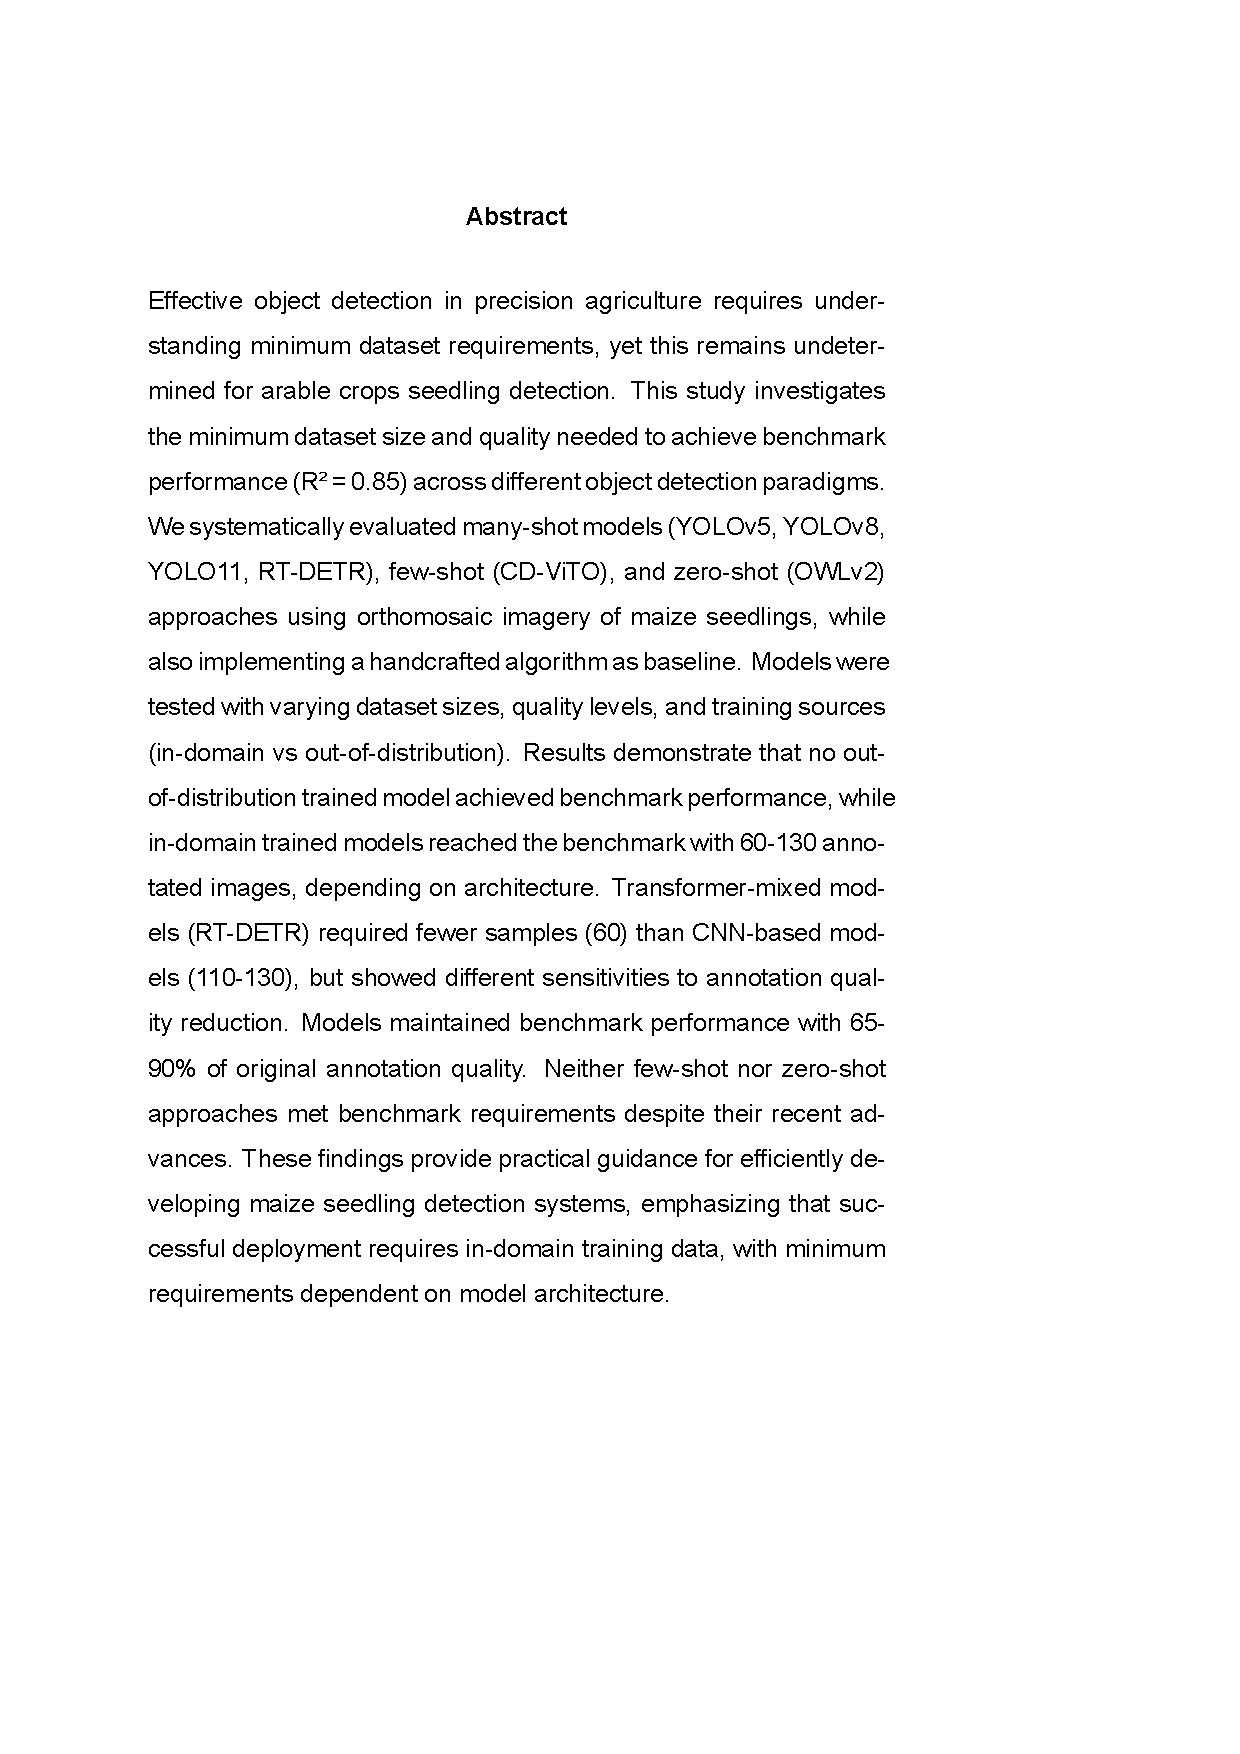
\includepdf[pages=-]{Plant_count.pdf}

\section{Ordinal and Nominal Variables}
\subsection{Phytoxicity Score}


\includepdf[pages=-]{Phytotoxicity_score/Phytoxicity_score.pdf}

\section{Binary Variables}
\subsection{Embedding Spaces for Control Sample Anomaly Detection}

\bibliographystyle{plainnat}
\bibliography{Phd_Thesis_SBumbaca}

\end{document}
